\documentclass[oneside]{Style/cugthesis}%
% \documentclass[twoside]{Style/cugthesis}%
\usepackage{caption}
\usepackage[super,numbers, list,table,math]{Style/artratex}

\usepackage{Style/artracom}% user defined commands

%%%%%%  change \DEGREE{} to select template %%%%%
\DEGREE{Master} % Master | MasterFull | Doctor
%
\schoolcode{10491}
\studentID{12022XXXXX}
%%%%%%%%%%%%%%%%%%%%%%%%%%%  中文封面 %%%%%%%%%%%%%%
\title{中文论文题目}% 论文中文题目
\author{论文作者}
\advisor{XXX~教授}% 指导教师:姓名 专业技术职务 工作单位
% \advisor{指导教师一\\指导教师二\\指导教师三}% 多行指导教师示例
\degree{硕士} % should be consistent with \DEGREE{}, 硕士 | 博士
\major{数学}
\institute{数学与物理学院}
\date{2025}{6} % 毕业时间

%%%%%%%%%%%%%%%%%%%%%%%%%%%  英文封面 %%%%%%%%%%%%%%
\TITLE{Title of the Thesis}
\AUTHOR{XXX~XX}% 论文作者
\ADVISOR{Prof.~XXX~XX}% 指导教师
% \ADVISOR{Teacher1\\Teacher2\\Teacher3}% 多行指导教师示例
\MAJOR{Mathematics}
\DEGREETYPE{Science}
%---------------------------------------------------------------------------%

\begin{document}

% 关于 \frontmatter 相关命令解释:https://www.zhihu.com/question/56203547
\frontmatter% initialize the environment

%%%%%%%%%%%%%%%%%%% Title page, declaration, author CV, abstract %%%%%%%%%%%
\maketitle% 生成中文封面
\MAKETITLE% 生成英文封面
\makedeclaration% 生成声明页
\maketeacherdeclaration% 生成声明页
\makeip% 授权页
\input{Tex/cv}
\makeabstractname{摘\quad 要}% 显示在书签但不显示在目录

这是中文摘要

\keywords{中国地质大学(武汉),学位论文,模板}% 中文关键词

\makeabstractname{Abstract}% 显示在书签但不显示在目录

This is abstract (en)

\KEYWORDS{China University of Geosciences, Wuhan, Thesis, LaTeX Template}% 英文关键词

\pagestyle{empty}%
\cleardoublepage\pagestyle{empty}%
%---------------------------------------------------------------------------%


%%%%%%%%%%%%%%%%%%% Table of content %%%%%%%%%%%%%%%%%%%%%%%
{
\linespread{1.2}% local line space
\contenttobmk
\newpage

\begin{center}
\tableofcontents
\end{center}

% \intobmk*{\cleardoublepage}{图表目录}
% \pagestyle{noheaderstyle}
% {
\cleardoublepage
{
\let\clearpage\relax  % Do nothing when a \clearpage command appears 
\let\cleardoublepage\relax

\renewcommand*{\addvspace}[1]{}
\let\oldnumberline\numberline%
\renewcommand{\numberline}{\figurename~\oldnumberline}%

\listoffigures
\let\clearpage\relax  % Do nothing when a \clearpage command appears 
\let\cleardoublepage\relax
\renewcommand{\numberline}{\appfigname~\oldnumberline}%
\vspace{-30pt}
\listofappfigs
}
{

\let\clearpage\relax  % Do nothing when a \clearpage command appears 
\let\cleardoublepage\relax
\renewcommand*{\addvspace}[1]{}
\let\oldnumberline\numberline%
\renewcommand{\numberline}{\tablename~\oldnumberline}%
\listoftables

\renewcommand{\numberline}{\apptabname~\oldnumberline}%
\vspace{-30pt}
\listofapptabs
}


}
% \thispagestyle{empty}

% % \intobmk*\chapter*{符号列表}% 显示在书签但不显示在目录
\makesymbollist


\section*{字符}
\nomenclatureitem[\textbf{Unit}]{\textbf{Symbol}}{\textbf{Description}}
\nomenclatureitem[$\Unit{m^{2} \cdot s^{-2} \cdot K^{-1}}$]{$R$}{the gas constant}
\nomenclatureitem[$\Unit{m^{2} \cdot s^{-2} \cdot K^{-1}}$]{$C_v$}{specific heat capacity at constant volume}
\nomenclatureitem[$\Unit{m^{2} \cdot s^{-2} \cdot K^{-1}}$]{$C_p$}{specific heat capacity at constant pressure}
\nomenclatureitem[$\Unit{m^{2} \cdot s^{-2}}$]{$E$}{specific total energy}
\nomenclatureitem[$\Unit{m^{2} \cdot s^{-2}}$]{$e$}{specific internal energy}
\nomenclatureitem[$\Unit{m^{2} \cdot s^{-2}}$]{$h_T$}{specific total enthalpy}
\nomenclatureitem[$\Unit{m^{2} \cdot s^{-2}}$]{$h$}{specific enthalpy}
\nomenclatureitem[$\Unit{kg \cdot m \cdot s^{-3} \cdot K^{-1}}$]{$k$}{thermal conductivity}
\nomenclatureitem[$\Unit{kg \cdot m^{-1} \cdot s^{-2}}$]{$S_{ij}$}{deviatoric stress tensor}
\nomenclatureitem[$\Unit{kg \cdot m^{-1} \cdot s^{-2}}$]{$\tau_{ij}$}{viscous stress tensor}
\nomenclatureitem[$\Unit{1}$]{$\delta_{ij}$}{Kronecker tensor}
\nomenclatureitem[$\Unit{1}$]{$I_{ij}$}{identity tensor}

\section*{算子}
\nomenclatureitem{\textbf{Symbol}}{\textbf{Description}}
\nomenclatureitem{$\Delta$}{difference}
\nomenclatureitem{$\nabla$}{gradient operator}
\nomenclatureitem{$\delta^{\pm}$}{upwind-biased interpolation scheme}

\section*{缩写}
\nomenclatureitem{CFD}{Computational Fluid Dynamics}
\nomenclatureitem{CFL}{Courant-Friedrichs-Lewy}
\nomenclatureitem{EOS}{Equation of State}
\nomenclatureitem{JWL}{Jones-Wilkins-Lee}
\nomenclatureitem{WENO}{Weighted Essentially Non-oscillatory}
\nomenclatureitem{ZND}{Zel'dovich-von Neumann-Doering}

% symbol list, preface content
}

\mainmatter% initialize the environment

%---------------------------------------------------------------------------%
%->> Main content
%---------------------------------------------------------------------------%
\renewcommand{\thefigure}{\thechapter.\arabic{figure}}
\renewcommand{\thetable}{\thechapter.\arabic{table}}
\renewcommand{\theequation}{\thechapter.\arabic{equation}}
\renewcommand{\mathbb}{\mathbbalt} % 修改默认 \mathbb 字体

{
% \let\cleardoublepage\relax % you can use this command to disable \cleardoublepage

\chapter{LaTeX使用说明}\label{chap:chapter1}
{
章引,本章主要分析XXXX.

\section{图表使用}

插入 pdf 图片,如图 \ref{fig:figure1} 所示.
\begin{figure}[!htbp]
    \centering
    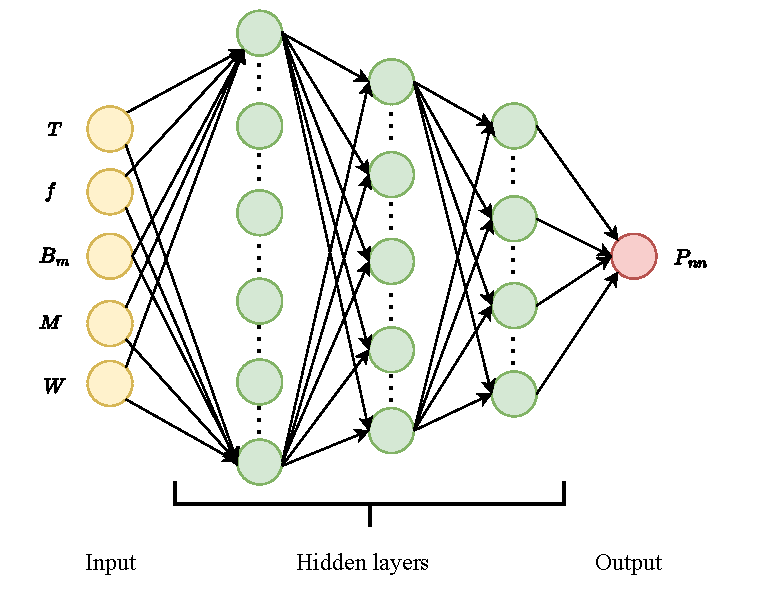
\includegraphics[width=0.40\textwidth]{figure1}
    \caption{插入 pdf 图片.}
    % \bicaption{\enspace 样图}{\enspace Sample Figure}
    % \fignote{对图片的注释}
    \label{fig:figure1}
\end{figure}

插入 png 图片,如图 \ref{fig:figure2} 所示.
\begin{figure}[!htbp]
    \centering
    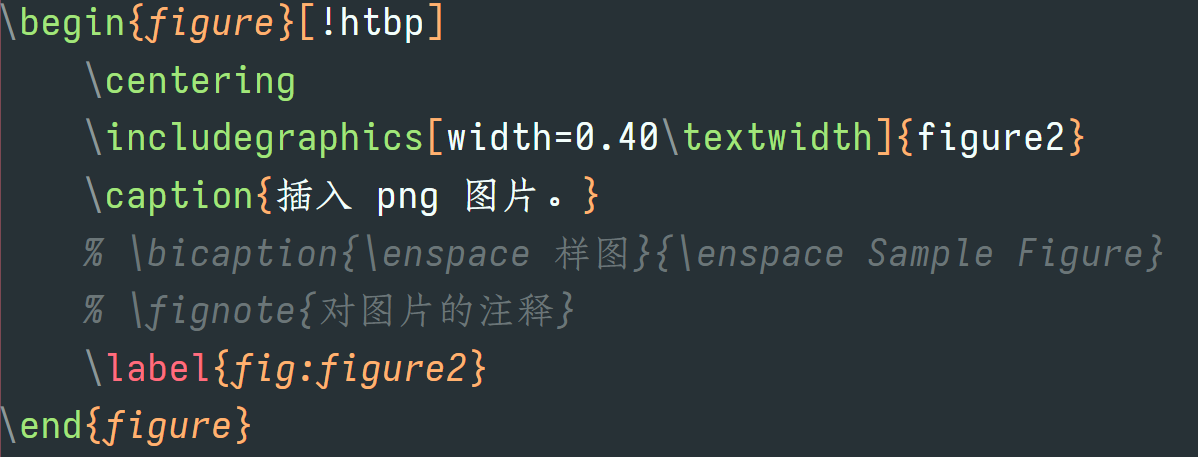
\includegraphics[width=0.40\textwidth]{figure2}
    \caption{插入 png 图片.}
    % \bicaption{\enspace 样图}{\enspace Sample Figure}
    % \fignote{对图片的注释}
    \label{fig:figure2}
\end{figure}

三线表设置,如表 \ref{tab:table1} 所示.
\begin{table}[!htbp]
    % \bicaption{\enspace 这是一个样表}{\enspace This is a sample table}
    \caption{插入三线表,表中字号设置为 \textbf{\backslash footnotesize}, 默认为 5 号字.}
    \label{tab:table1}
    \centering
    \footnotesize% fontsize
    \setlength{\tabcolsep}{4pt}% column separation
    % \renewcommand{\arraystretch}{1.2}%row space 
    \begin{tabular}{lcccccccc}
        \toprule
        行号 & \multicolumn{8}{c}{跨多列的标题}\\
        %\cline{2-9}% partial hline from column i to column j
        \midrule
        Row 1 & $1$ & $2$ & $3$ & $4$ & $5$ & $6$ & $7$ & $8$\\
        Row 2 & $1$ & $2$ & $3$ & $4$ & $5$ & $6$ & $7$ & $8$\\
        Row 3 & $1$ & $2$ & $3$ & $4$ & $5$ & $6$ & $7$ & $8$\\
        Row 4 & $1$ & $2$ & $3$ & $4$ & $5$ & $6$ & $7$ & $8$\\
        \bottomrule
    \end{tabular}
\end{table}

有序列表:
\begin{enumerate}
    \item item1.
    \item item2.
\end{enumerate}

无序列表:
\begin{itemize}
    \item item1.
    \item item2.
\end{itemize}

公式:
\begin{equation}
    \boldsymbol{y} = f(\boldsymbol{x}) + \boldsymbol{\varepsilon}, \boldsymbol{x}\in\mathbb{R}^n, \label{eq:equation1}
\end{equation}
见式~\eqref{eq:equation1}.

参考文献引用格式\cite{journal, inproceedings, book}.

\vspace*{2cm}
{\colorbox[rgb]{0.9,0.6,0.2}{本模板根据中国科学院大学模板修改得到,具体可查看此链接:}}

{\colorbox[rgb]{0.9,0.6,0.2}{\href{https://github.com/mohuangrui/ucasthesis}{https://github.com/mohuangrui/ucasthesis}.}}


}
}

%---------------------------------------------------------------------------%
% !!! MAIN CONTENT

\intotoc*{\cleardoublepage}{\bibname}% add link to toc
\artxifstreq{\artxbib}{bibtex}{% enable bibtex
    \bibliography{Biblio/ref}% bibliography
}{%
    \printbibliography% bibliography
}

\cleardoublepage[plain]%

%%%%%%%%%%%%%%%%%%%%%%%%%%%%%%%%%%%%%%%%%%%%%%%  appendix %%%%%%%%%%%%%%
% \appendix% initialize the environment
% \stepcounter{app}
\setcounter{app_fig}{1}
\setcounter{app_tab}{1}
\setcounter{equation}{0}
\renewcommand\theequation{附\arabic{app}-\arabic{equation}}
% \renewcommand\theequation{\Alph{app}.\arabic{equation}}
\renewcommand\chaptername{附录}
\renewcommand\chaptername{Appendix} 
\renewcommand\thechapter{附录\zhnum{app}} 

\setcounter{chapter}{0}
\setcounter{section}{0}
\chapter{附录中的公式}\label{chap:app1}{

%%% START HERE
\begin{equation} \label{eq:appedns}
    % \adddotsbeforeeqnnum%
    \begin{cases}
        \frac{\partial \rho}{\partial t} + \nabla\cdot(\rho\Vector{V}) = 0\\
        \frac{\partial (\rho\Vector{V})}{\partial t} + \nabla\cdot(\rho\Vector{V}\Vector{V}) = \nabla\cdot\Tensor{\sigma}\\
        \frac{\partial (\rho E)}{\partial t} + \nabla\cdot(\rho E\Vector{V}) = \nabla\cdot(k\nabla T) + \nabla\cdot(\Tensor{\sigma}\cdot\Vector{V})
    \end{cases}
\end{equation}

\begin{equation} \label{eq:appedns2}
    % \adddotsbeforeeqnnum%
    \begin{cases}
        \frac{\partial \rho}{\partial t} + \nabla\cdot(\rho\Vector{V}) = 0\\
        \frac{\partial (\rho\Vector{V})}{\partial t} + \nabla\cdot(\rho\Vector{V}\Vector{V}) = \nabla\cdot\Tensor{\sigma}\\
        \frac{\partial (\rho E)}{\partial t} + \nabla\cdot(\rho E\Vector{V}) = \nabla\cdot(k\nabla T) + \nabla\cdot(\Tensor{\sigma}\cdot\Vector{V})
    \end{cases}
\end{equation}


mathtext: $A,F,L,2,3,5,\sigma$, mathnormal: $A,F,L,2,3,5,\sigma$, mathrm: $\mathrm{A,F,L,2,3,5,\sigma}$.

mathbf: $\mathbf{A,F,L,2,3,5,\sigma}$, mathit: $\mathit{A,F,L,2,3,5,\sigma}$, mathsf: $\mathsf{A,F,L,2,3,5,\sigma}$.

mathtt: $\mathtt{A,F,L,2,3,5,\sigma}$, mathfrak: $\mathfrak{A,F,L,2,3,5,\sigma}$, mathbb: $\mathbb{A,F,L,2,3,5,\sigma}$.

mathcal: $\mathcal{A,F,L,2,3,5,\sigma}$, mathscr: $\mathscr{A,F,L,2,3,5,\sigma}$, boldsymbol: $\boldsymbol{A,F,L,2,3,5,\sigma}$.

vector: $\Vector{\sigma, T, a, F, n}$, unitvector: $\unitVector{\sigma, T, a, F, n}$

matrix: $\Matrix{\sigma, T, a, F, n}$, unitmatrix: $\unitMatrix{\sigma, T, a, F, n}$

tensor: $\Tensor{\sigma, T, a, F, n}$, unittensor: $\unitTensor{\sigma, T, a, F, n}$ 

% \thispagestyle{appendixheader}
\cleardoublepage[plain]
}% appendix content

\backmatter% initialize the environment
%---------------------------------------------------------------------------%
%->> Backmatter
%---------------------------------------------------------------------------%
\chapter[致谢]{致\quad 谢}\chaptermark{致\quad 谢}% syntax: \chapter[目录]{标题}\chaptermark{页眉}
%\thispagestyle{noheaderstyle}% 如果需要移除当前页的页眉
%\pagestyle{noheaderstyle}% 如果需要移除整章的页眉

此处填写致谢。

\cleardoublepage[plain]% 让文档总是结束于偶数页,可根据需要设定页眉页脚样式,如 [noheaderstyle]
%---------------------------------------------------------------------------%
% other information

\end{document}










%---------------------------------------------------------------------------%

